\chapter{TPC Electronics}
\label{ch:fddp-tpc-elec}
%try to modify file


%%%%%%%%%%%%%%%%%%%%%%%%%%%%%%%%%%%%%%%%%%%%%%%%%%%%%%%%%%%%%%%%%%%%
\section{TPC Electronics System Overview}
\label{sec:fddp-tpc-elec-ov}

%%%%%%%%%%%%%%%%%%%%%%%%%%%%%%%%%
\subsection{Introduction}
\label{sec:fddp-tpc-elec-intro}

The charge readout system is designed to provide continuous, non-zero-suppressed, and losslessly compressed of \SI{3}{m} long strips arranged in two collection views with a pitch of \SI{3.125}{mm} in the Charge Readout Planes (CRPs) of a dual-phase detector module. The goals of the DP TPC electronics is to collect and digitize the signals from the Charge Readout Plane (CRP) and photon detectors, Photo-Multiplier Tubes (PMT), in the Dual-Phase TPC. The system is built from the components already developed for the ProtoDUNE-DP detector. Compared to ProtoDUNE-DP, a single DP detector module has a factor of 20 more readout (both charge and light) channels. The modular structure of incorporated the design ... 

The scaling ...  
The system for the charge readout consists of a Front-End (FE) analog electronics operating at cryogenic temperatures and digital electronics working in the warm environment outside of the cryostat. The cold electronics are therefore accessible from the outside and optimum for the signal (short cables to reduce capacitance and low temperature to reduce noise).  The PMT signals, are not pre-amplified, but routed directly to the Light Read-Out electronics (LRO).

%The analog of light readout ... The digitization... Need to unify the description a bit... the anode PCBs of the Charge Readout Plane (CRP).

The FE analog electronics for Charge ReadOut (CRO) is based on cryogenic ASIC chip with a large dynamic range (up to \SI{1200}{fC}) to cope with the charge amplification in the dual-phase CRP. The FE cards are placed close to CRP and are accessible even after the detector module is filled with liquid argon. They are housed in dedicated Signal FeedThrough (SFT) chimneys, which are approximately \SI{2}{m} long objects that traverse the entire insulation layer of the cryostat.  The analog signals from the analog FE cards are brought out via the SFT interface to the digital electronics located on top of the cryostat support structure in the ambient environment of the detector module cavern. 

The digitization cards, Advanced Mezzanine Cards or AMCs, are housed in commercial uTCA crates. Each crate is connected to the DAQ system via an optical fiber link (at least \SI{10}{Gbit/s}). The uTCA crate also houses a module (WR-MCH) for the time synchronization of AMCs. This (slave) unit is connected via \SI{1}{Gbit/s} optical fiber to a master node that serves as a synchronization reference for all the connected slave nodes.  The time synchronization system is based on the commercially available components developed within the framework of the White Rabbit (WR) project. 

The detection of the direct scintillation light is the main purpose of the LRO electronics in order to provide the absolute interaction time of the events.
 The system will also be capable to detect the so-called proportional scintillation light produced by the electrons extracted and amplified in the gaseous phase. The actual photon detectors are assumed to be TPB-coated \num{8} inch photomultiplier tubes (Hamamatsu R5912-02-mod) located under the cathode. The number of photomultipliers assumed in the DUNE CDR was 180. This number of channels is likely to be increased by a factor 4 in order to have a similar or better surface coverage as in ProtoDUNE-DP. %objective? spe - 1000s?
%16 channel or 32 channel here?
The system will group up to 16 PMTs (32) to be read by a single AMC card in uTCA standard which architecture is derived from an adaptation of the charge readout cards. The different cards are inserted in uTCA crates and the events are time stamped using the White Rabbit system of the charge readout by including in each uTCA crate a White Rabbit slave node card.
%when to explain what info is being derived from LRO?

A small-scale version of the TPC CRO electronics system has been used in a small dual-phase LArTPC prototype at CERN with an active volume (CRP area) of $3\times 1 \times 1$ \si{\meter\cubed} ($3\times1$ \si{\meter\squared} operating in the Summer-Fall 2016. 
\fixme{Summarize main points of the electronics operation in 311 here.}

%\fixme{Include an image of the overall system, indicating its parts. Show how the system fits into the overall detector.}
%The operating principle is illustrated in Figure~\ref{figure-label}... (add figure)
%\begin{dunefigure}[optional caption for LoF]{fig:figure-label}
%{required full caption (Credit: xyz)}
%\includegraphics[width=0.8\textwidth]{image-filename}
%\end{dunefigure}

%%%%%%%%%%%%%%%%%%%%%%%%%%%%%%%%%%%%%
\subsection{Design Considerations}
\label{sec:fddp-tpc-elec-des-consid}

The design of the electronics for the charge readout covers the analog front-end cards containing pre-amplifier ASICs operating at cryogenic temperatures and digitization cards with the relevant system for their synchronization working in the warm environment outside of the cryostat. The principle requirements for the system is to read and digitize signals from a total of \num{153600} channels (per one DP detector module) and be capable of continuously streaming the collected and losslessly compressed data to DAQ without any zero suppression. Given the amplification of the charge in CRP, the electronics needs to be sensitive to the signals over a large dynamic range (up-to \num{40} times the MIP-level signals for a nominal CRP gain of \num{20}) to avoid saturation of the analog inputs by large localized energy disposition generated in hadronic shower events. The charge amplification provided by the CRP loosens requirements on the intrinsic noise of the FE analog electronics. For the CRP nominal gain of \num{20}, the signal-to-noise ratio for a MIP signal (\SI{30}{fC}) should be at around \num{100}, which would not pose any problem for the detection/reconstruction. The magnitude of noise, however, plays a role in the quality of the lossless compression on the raw data performed by the digital electronics. A compression factor of \num{10} can be achieved with the noise levels below \num{1} ADC RMS.  %be careful of RMS<1...

%\fixme{The design of the electronics for the light readout covers ... The electronics must be able to read signals from \num{720} channels (per one DP detector module) and stream data continuously to the DAQ back-end. ...}
The primary objective of the Light Read Out system is to detect signals, from a minimum of one photoelectron on one PMT, giving a precise timestamp that can be used in conjunction with the Charge signals to determine the drift (z) co-ordinate of the event.  Precise measurements of signal charge will allow the continual monitoring of the PMT gain at the single photoelectron level, and the determination of the number of photons in each scintillation event.  In addition, an ADC will continuously stream data, downsampled to \SI{400}{ns} as for the Charge signals,  which, amongst other items, will allow measurements of the scintillation time-profile. 


The cryogenic analog electronics for charge readout is housed in SFT chimneys. Their design must enable access to the FE card for possible maintenance/replacement without any risk of contaminating the pure liquid argon in the main cryostat volume. The chimneys must possess a cooling system that would permit to control the temperature around the FE cards around \SI{110}{\kelvin} for their optimal noise. In addition, the cooling system is to compensate for the heat input from the chimney into the cryostat volume.

The digital electronics (for both charge and light readout) is located at warm on the roof of the cryostat supporting structure and is therefore easily accessible placing. The fact removes any constraints associated with accessibility and environmental conditions and allows for the usage of the standard components and industrial solutions in its design. Digital electronics must be continuously and automatically synchronized to better than \SI{400}{ns} to ensure the correct temporal alignment of the ADC samples from all of the readout channels. This requirement derives from the fact the sampling rate of the temporal coordinate (along the drift direction) is \SI{2.5}{\MHz}. 

Some of the key parameters in the electronics system design are summarized in Table~\ref{tab:dp-elecphysicsparams}.

\begin{dunetable}
[Parameters for the TPC electronics system design]
{lr}
{tab:dp-elecphysicsparams}
{Parameters for the  TPC electronics system design. The numbers are given for one detector module.}   
Parameter & Value  \\ \toprowrule
  Charge readout channels    &  \num{153600}            \\ \colhline
  Charge readout continuous sampling rate & \SI{2.5}{\MHz}\\ \colhline
  Charge readout ADC resolution & \num{12} bit           \\ \colhline
  Charge readout data compression factor   & \num{10}    \\ \colhline 
  Charge readout data flow  & \num{430} Gbit/s          \\ \colhline 
  Light readout channels       & \num{720}               \\ \colhline
  Light readout continuous sampling rate & \SI{2.5}{\MHz} \\ \colhline
  Light readout ADC resolution & \num{14} bit            \\ \colhline
  Light readout data compression factor  & \num{1}       \\ \colhline
  Light readout data flow   & \num{24} Gbit/s          \\ \colhline
\end{dunetable}

%\fixme{Anne suggests: Within this section add ref to requirements document  when it's ready, and maybe list the most important half dozen in a table here). E.g.,}  
%\fixme{By the end of the volume, for every requirement listed in this section, there should exist an explanation of how it will be satisfied.}


%%%%%%%%%%%%%%%%%%%%%%%%%%%%%%%%
\subsection{Scope}
\label{sec:fddp-tpc-elec-scope}

The scope of the TPC electronics system covers the procurement and productions, testing and validation, installation, and commissioning of all the components necessary to ensure the complete readout of the charge and light signals from a given DP detector module. The covered items are the following:
\begin{itemize}
\item{Cryogenic analog FE cards for charge readout}
%\item{Analog electronics for the light readout\fixme{more details/names?}}
\item{Digital AMC cards for charge/light readout}
\item{The WR-MCH cards for AMC clock synchronization}
\item{uTCA crates}
\item{Switches for the White Rabbit network}
\item{SFT chimneys}
\item{Low-voltage power supplies for the FE cards}
\item{Flat cables connecting the FE cards to the warm flange interface of the SFT chimneys}
\item{VHDCI cables connecting the warm flange interface of the SFT chimneys to AMCs}
\end{itemize}



%%%%%%%%%%%%%%%%%%%%%%%%%%%%%%%%%%%%%%%%%%%%%%%%%%%%%%%%%%%%%%%%%%%%
\section{TPC Electronics System Design}
\label{sec:fddp-tpc-elec-design}

The FE analog electronics for charge readout is based on cryogenic ASIC chip with a large dynamic range ($0-1200$ \si{fC}) to cope with the charge amplification in the dual-phase CRP. The FE cards read \num{64} channel CRP channels each. They are mounted in dedicated Signal FeedThrough (SFT) chimneys and are located within a short distance ($\sim$\SI{1}{\metre}) from CRP to minimize the noise caused by long cables (large cable capacitance). The cards remain accessible throughout the detector operation. Each SFT chimney hosts nominally \num{10} FE analog cards, which corresponds to the readout of \num{640} CRP channels per chimney. There are, therefore, \num{240} SFT chimneys to be installed for the charge readout in a given DP detector module.   

The differential analog signals from the analog FE cards, routed via an interface flange of SFT, are digitized by AMC cards located at warm outside of the cryostat. AMCs are hosted in uTCA crates. In the baseline version of the design (utilized currently in ProtoDUNE-DP), each AMC digitizes \num{64} channels corresponding to reading one FE analog card. Each uTCA in such case contains \num{10} AMCs (\num{640} channel). However, an implementation with AMCs supporting a higher channel density is also being investigated for cost reduction purposes. 

\fixme{Layout the light readout design... Then we should give unified description of uTCA crates.}

A given SFT chimney is serviced by one uTCA crate placed in its immediate vicinity. In addition to the digitization cards, the uTCA crates also contain an network switch (MCH) via which the digitized data is to be sent to DAQ and a module for clock/time synchronization and trigger timestamp distribution of the AMCs (WR-MCH). Both MCH and WR-MCH require one optical fiber link each. 

The MCH (MicroTCA Carrier Hub) switch transmits the data from AMCs via a dedicated optical link. Currently ProtoDUNE-DP uses MCH operating at 10 Gbit/s. However, a move to 40 Gbit/s links for the DUNE FD implementation is considered because of the technology evolution and possible increase in the channel density of each AMC.

The WR-MCH time synchronization unit is based White Rabbit (WR) system, which provides hardware and protocols for the network-based sub-ns synchronization between a master and different slave nodes. The connection of the WR-MCH to the White Rabbit network is done via \num{1}\si{Gbit/s} optical link. WR-MCH distributes the timing information for synchronization to the AMCs via the uTCA backplane. In addition, this unit can be used to transmit triggers to the digitization units within the crate. This is achieved by sending it dedicated data packets containing trigger timestamp information. 

Figure~\ref{fig:dune10ktdp} shows the top part of the cryostat warm structure with the pattern of the SFT chimneys and uTCA crates. A cut-out view of the chimney illustrates the location of the FE cards and provides the overall scale of this object. 

\fixme{Other picture for light readout? ...}
\fixme{show pictures of which parts of CRP a given chimney reads}

\begin{dunetable}
[Summary of some of the principal numbers of the TPC electronics system.]
{lr} {tab:dpele-numparts}
{Summary of some of the principal numbers of the TPC electronics system for charge and light readout of a detector module}
Name & Number  \\ \toprowrule
   SFT chimneys/uTCA crates              &  \num{240}   \\ \colhline
   Channels per SFT chimney/uTCA crate & \num{640} \\ \colhline
   Cryogenic analog FE cards per SFT chimney    &  \num{10}     \\ \colhline
   Cryogenic analog FE cards (total)                   & \num{2400}  \\ \colhline
   Charge readout AMCs per uTCA crate                       & \num{10}      \\ \colhline
   Charge readout AMCs (total)                                   & \num{2400}      \\ \colhline 
   Light readout FE cards  per uTCA crate & \num{9} \\ \colhline
   Light readout FE cards (total)           & \num{45} \\ \colhline
   Light readout channels per uTCA crate & \num{144} \\ \colhline
   WR-MCH per uTCA crate                 & \num{1} \\ \colhline
   WR-MCH (total)                              & \num{245} \\ \colhline
   uTCA crates (total)                         & \num{245} \\ \colhline
\end{dunetable}

A short summary of some of the principal number such as components and channel granularity in the design of the DP electronics is provided in Table~\ref{tab:dpele-numparts}. 

%%%%%%%%%%%%%%%%%%%%%%%%%%%%%%%%%%%
\subsection{Cryogenic Analog FE Electronics}
\label{sec:fddp-tpc-elec-design-cryofe}

The cryogenic amplifer ASIC is the principle component of the FE analog cards. Their design is based on the CMOS \SI{0.35}{\micro\meter} technology and is an outcome of an R\&D  activity started in 2006. Two principal version of ASIC chips have been produced for the dual-phase LArTPC operation. In the first version the amplifiers have a constant gain in the region of $0-1200$ \si{\femto\coulomb} ($0-40$ MIP). In the second one, they have a higher linear gain for signals up to \SI{400}{\femto\coulomb} (roughly 10 MIP signals) and a logarithmic response in the  $400-1200$ \si{\femto\coulomb} range. This double-slope behavior is obtained by using a MOSCAP capacitor in the feedback loop of the amplifier that changes its capacitance above a certain signal threshold. The aim of this solution is optimize the resolution for small charge depositions (in a few MIP region) while preserving the large dynamic range of the amplifier. Figure~\ref{fig:dpele-fe-asic-gain} illustrates the amplifier gain as a function of the injected charge for the two ASIC design. The ASIC version with the double-slope gain has been selected for ProtoDUNE-DP. 

\begin{dunefigure}[Gain of the cryogenic FE ASIC]{fig:dpele-fe-asic-gain}
{Gain of the cryogenic FE ASIC}
%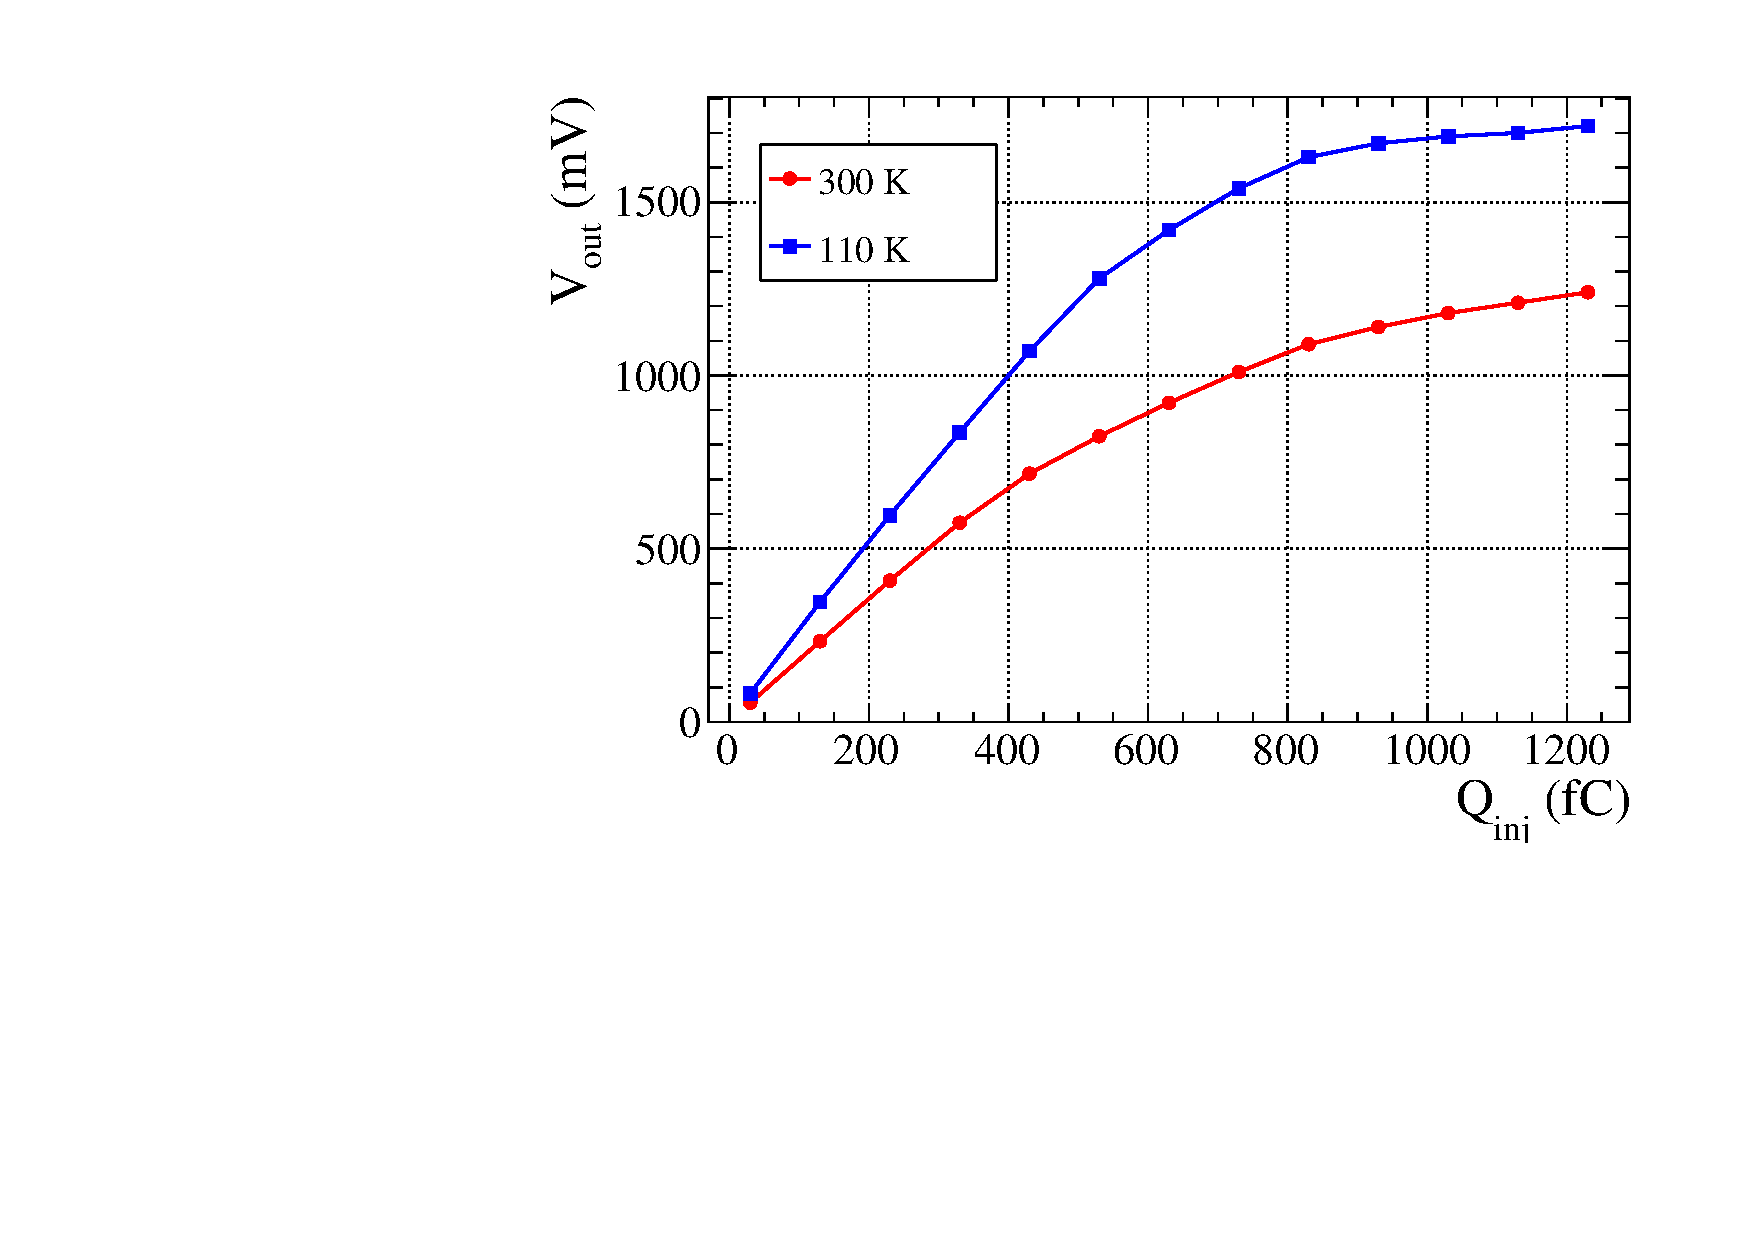
\includegraphics[width=0.5\textwidth]{dpele-fe-asic-gain}
\end{dunefigure}

Each ASIC contains 16 amplifier channels with differential line buffers and has a power consumption which is $<18$ mW per channel. The measured noise as a function of the input ("detector")  capacitance is shown in Figure~\ref{fig:dpele-fe-asic-noise} for different temperatures.  

\begin{dunefigure}[Noise of the cryogenic FE ASIC as a function the detector capacitance]{fig:dpele-fe-asic-noise}
{Noise of the cryogenic FE ASIC as a function the detector capacitance}
%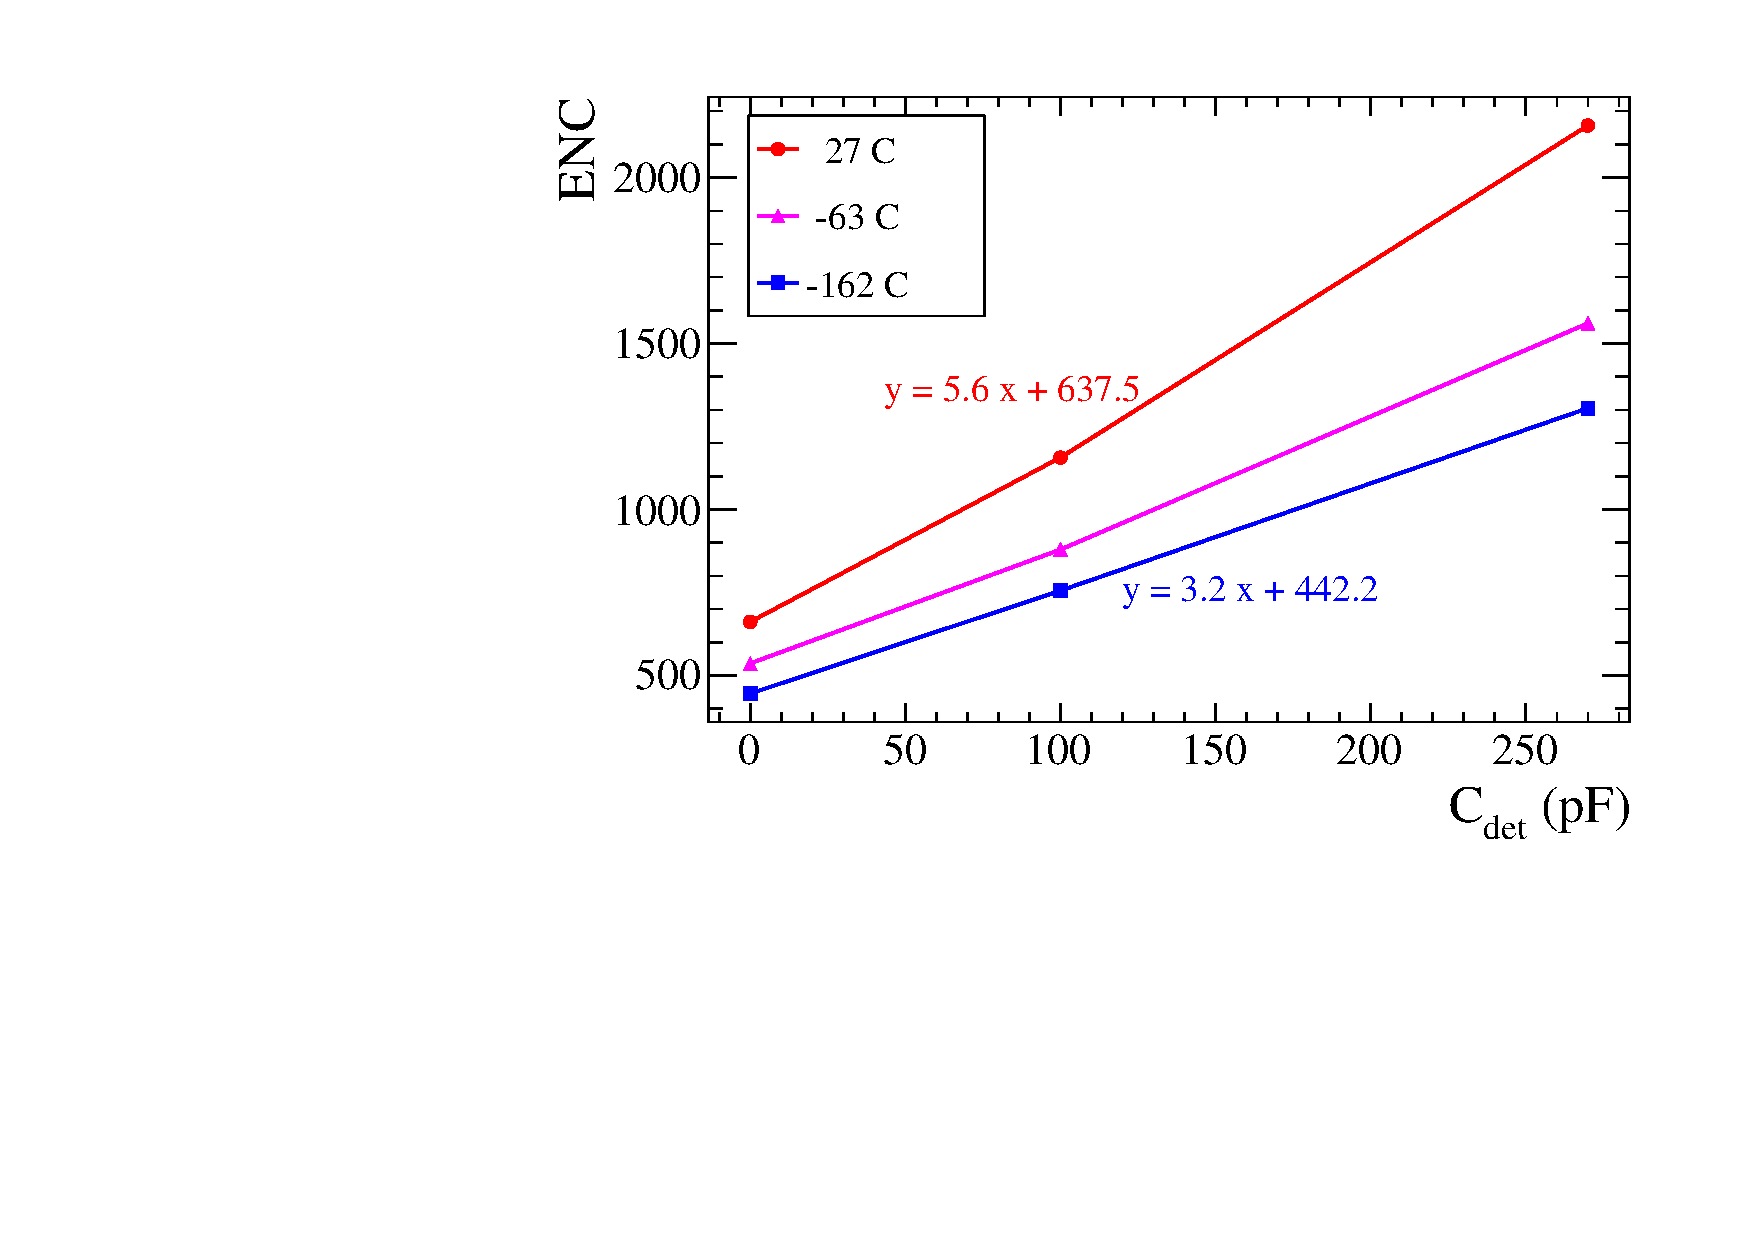
\includegraphics[width=0.5\textwidth]{dpele-fe-asic-noise}
\end{dunefigure}

\begin{dunefigure}[Image of an analog FE card from ProtoDUNE-DP]{fig:dpele-fe-card-image}
{Image of an analog cryogenic FE card from ProtoDUNE-DP}
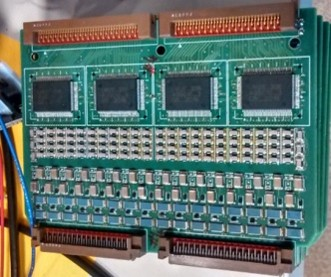
\includegraphics[width=0.5\textwidth]{dpele-fe-card-image}
\end{dunefigure}

Each cryogenic FE card, shown in Figure~\ref{fig:dpele-fe-card-image}, hosts 4 ASIC amplifier chips and a few passive discrete components. The input stage of each amplifier channel has a \SI{1}{\giga\ohm} resistor to ground followed by a \SI{2.2}{\nano\farad} decoupling capacitor. The function of the resistor is to provide the ground reference for the anode strips of CRP. Each input stage is protected against discharges coming from the detector with a TVS diode (Bourns CDSOD323-T08LC). This component was selected after studying the performance of different ESD components subjected systematically to discharges of a few kV with an energy similar to that of LEMs in CRP. The FE cards also house the blocking capacitors for filtering the low voltage power lines.


%%%%%%%%%%%%%%%%%%%%%%%%%%%%%%%%%%%
\subsection{SFT Chimneys}
\label{sec:fddp-tpc-elec-design-sft}

The SFT chimneys are designed to enable the access to the FE analog electronics for a potential repair or exchange while the detector is in operation (filled with the liquid argon). In addition, their metallic structure acts as a Faraday cage isolating the FE ASICs from environmental interference.  Each SFT nominally hosts \num{10} analog cryogenic FE cards (reading \num{640} channels in total).  Some of the details of the design are illustrated in Figure~\ref{fig:dpele-sft-chimney-design}. 

\begin{dunefigure}[Details of the SFT chimney design]{fig:dpele-sft-chimney-design}
{Details of the SFT chimney design}
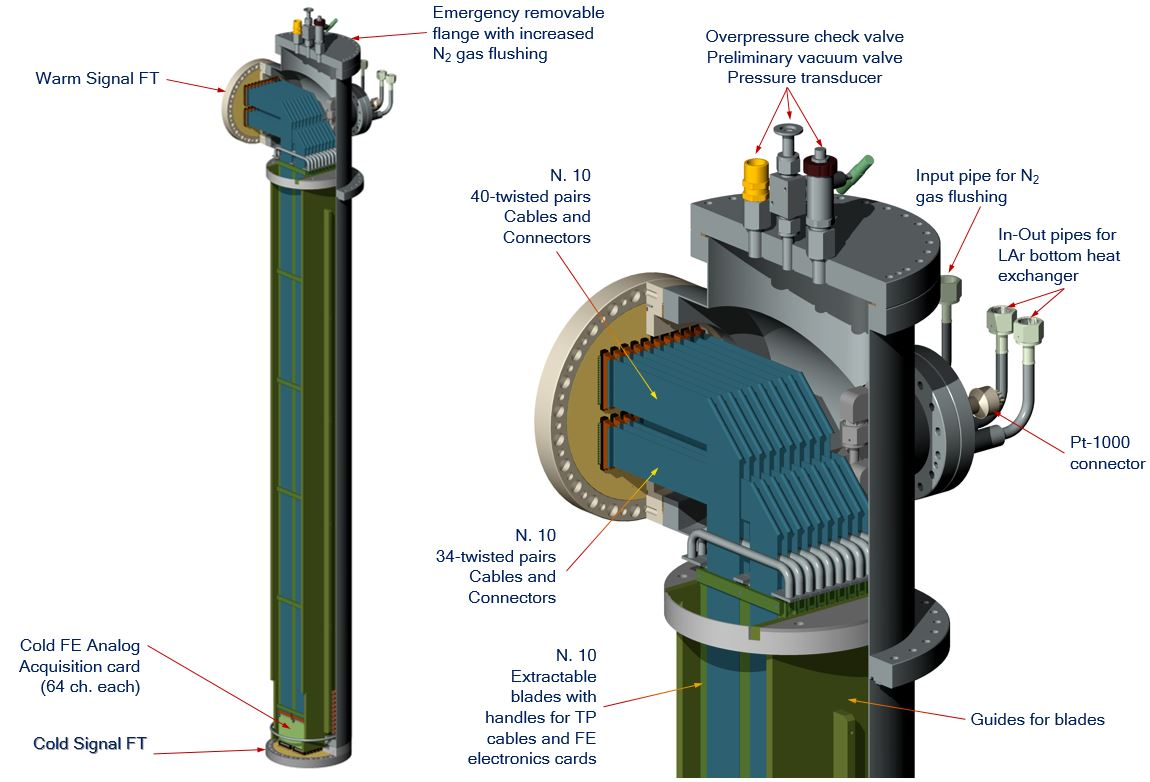
\includegraphics[width=0.8\textwidth]{dpele-sft-chimney-design}
\end{dunefigure}

The chimneys are closed at the bottom and top with vacuum tight flanges whose function is to dispatch the signal and slow control lines. The flange at the bottom, cold flange, isolates (ulta-high vacuum tightness standard) the inner volume of the detector module from the chimney volume and interconnects the signals from the CRP to the analog FE cards. The flange at the top, warm flange, seals the chimney from the outside environment. It also passes the low voltage and control lines to the FE electronics inside and brings out the differential analog signal lines from the FE amplifiers. 

The SFT chimney volume is filled with nitrogen gas at near atmospheric pressure. The temperature inside the chimney could be adjusted using a heat exchanger coil cooled with liquid argon. It is located at the bottom close to the cold flange around the FE cards. The functions of this cooling system are to mitigate the heat input to the main detector volume and provide optimal (lowest noise) operating temperature for the FE electronics of around \SI{110}{K}. A pressure release valve, indicated in Figure~\ref{fig:dpele-sft-chimney-design}, protects the structure from an accidental overpressure in the inner volume. 

The expected heat input from a given SFT chimney is about \SI{20}{\watt}. This number includes the heat through the twisted-pair cables connected to the warm flange, the SFT outer metallic tube, as well as the heat dissipation by the FE cards. A total heat input from all \num{240} SFT chimneys is at the level of \SI{5}{\kilo\watt}. 

\begin{dunefigure}[Details of the SFT flange connections]{fig:dpele-sft-flanges}
{SFT cold flange with the FE cards inserted}
%\includegraphics[width=0.8\textwidth]{dpele-sft-flanges}
\end{dunefigure}

The analog FE cards are inserted directly onto the cold flange (see Figure~\ref{fig:dple-sft-flanges}). The other side of the flange (facing inside the cryostat) hosts the connectors for the flat cables coming from the CRP anodes.  The FE cards are mounted on \SI{2}{m} long blades made from FR4 \todo{check}, which enable the insertion/extraction of the electronics and also support the flat cables carrying signals, low voltages, and slow control to/from the warm flange interface.  The blades slide along the rails installed inside the chimney at opposite sides, which guide the FE cards to their respective connectors on the cold flange. 

Prior to the commissioning of a detector module, the chimneys are evacuated a dedicated KF16 \todo{check} port (see Figure~\ref{fig:dpele-sft-chimney-design}) and then filled with nitrogen gas. This ensures the removal of the moisture that would otherwise condense, once the detector module is filled with the liquid argon, around the FE cards damaging the electronics. To access the FE cards once the detector module is at cold, the stainless steel flange at the top of the SFT chimney (Figure~\ref{fig:dpele-sft-chimney-design}) must be removed. This procedure requires continuous flushing of nitrogen gas at slight over-pressure with respect to the atmospheric in order to prevent the humid air entering and generating condensation inside the chimney. Once a chimney is opened, the blades with the FE cards can be extracted after unplugging the flat cables (two per card) connected on the inner side of the warm flange (Figure~\ref{fig:dpele-sft-chimney-design}).

The procedure to access the FE cards at cold was successfully tested during the operation of the LArProto detector. The temperature at the top of the chimney was very close to the room temperature allowing to manipulate the cable connections one warm flange without any cryogenic gloves. The movement of the blades on the rails and the FE card extraction / insertion did not indicate any mechanical problems that could have been caused by shrinking of various elements due to the lower temperatures.  The signals from the FE cards that underwent the extraction/insertion were also checked and no malfunctioning channels were found.

%%%%%%%%%%%%%%%%%%%%%%%%%%%%%%%%%%%
%\subsection{Low-voltage Power Supplies for FE Electronics}
%\label{sec:fddp-tpc-elec-design-lvps}

%%%%%%%%%%%%%%%%%%%%%%%%%%%%%%%%%%%
\subsection{Digital AMC Electronics}
\label{sec:fddp-tpc-elec-design-amc}

The function of the AMC cards is to read and digitize the data from the FE amplifier and then transmit them to the DAQ system. Each card has eight ADC chips (AD9257), two dual-port memories (IDT70T3339), and an FPGA (ALTERA Cyclone V) on board. The FPGA provides a virtual processor (NIOS) that handles the readout and the data transmission.  The cards also include a last stage of analog shaping before the ADC input.

\begin{dunefigure}[Block diagram of AMC]{fig:dpele-amc-scheme}
{Block diagram of AMC}
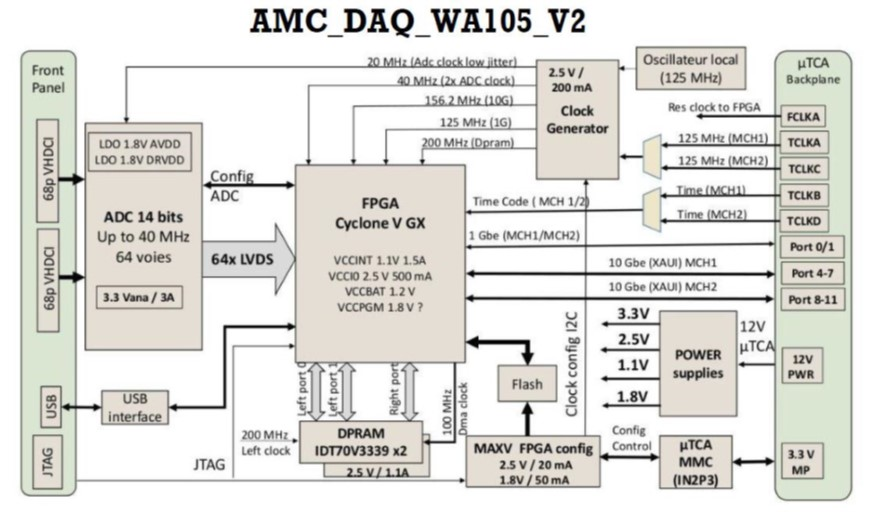
\includegraphics[width=0.7\textwidth]{dpele-amc-scheme}
\end{dunefigure}

Figure~\ref{fig:dpele-amc-scheme} shows block diagram of the AMC functionality. The data are continuously sampled at \SI{2.5}{\MHz} with \num{14} bit resolution. However only \num{12} most significant bits of each sample are eventually sent to the DAQ. Within AMCs lossless data compression based on an optimized version of the Huffman algorithm is performed and the data are organized in frames for transmission. The frames contain the absolute timing information of the first data sample.  In the current design, each AMC has 64 channels and reads one analog FE cards.

The AMCs are housed in uTCA crates and send their data via the MCH switch. The timing synchronization of AMCs is achieved via a WR-MCH module (also housed in the crate) that is connected to the White Rabbit network. In addition, WR-MCH could also be used for triggered readout of AMCs by sending it dedicated packets containing trigger timestamp information over the White Rabbit network.

In ProtoDUNE-DP, AMCs are operated in the triggered mode reading \SI{4}{\milli\second} drift time window at trigger rate of \SI{100}{Hz}, which is not far from a continuous readout mode. The digitized data are constantly recorded in a local memory buffer. A sub-sample of these data can then be acquired by providing AMC with a timestamp generated by an external trigger. The timestamp defines the start time for the data sequence to be retrieved from the buffer, while the length of the sequence is determined by the size of the drift window. In ProtoDUNE-DP this corresponds to \num{10000} (\SI{4}{\milli\second}) samples per full drift window.  Triggers (beam counters, cosmic ray counters, photomultipliers reading the UV light, starts of beam spills) are time stamped in a dedicated Whiter Rabbit slave node (WR-TSN), an FMC-DIO mezzanine mounted on WR SPEC carrier card, that runs a custom firmware and is hosted in a computer. The WR-TSN is connected to the WR Grand Master for synchronization and for transmission of the trigger information. The timestamp data produced by the WR-TSN are sent over the White Rabbit network as Ethernet packets with a customized protocol. 
   
%%%%%%%%%%%%%%%%%%%%%%%%%%%%%%%%%%%
\subsection{Network-based uTCA Architecture}
\label{sec:fddp-tpc-elec-design-utca}

The digital electronics is based on uTCA standard which offers industrial solution a very compact and easily scalable architecture to handle a large number of channels at low cost.  The standard (or related standards such as ATCA or xTCA) is widely used in the telecommunication industry and is being adapted by the HEP community. The backplane of the uTCA crates host high-speed serial links that support a variety of transmission protocols (Ethernet, PCI Express, SRIO, etc.). In addition, dedicated lanes are available for the distribution of the clock signals to all the boards hosted in the crate.  The Ethernet-based solution has been adopted for both the data and clock distribution in this design of the DP electronics system for both charge and light readout. 

Each AMC plugged into the uTCA is connected to the crate MCH board through the backplane serial links. The MCH provides the switch functionality that enables AMCs to communicate with each other or external systems through the MCH uplink interface. In the DP electronics system design, MCH also manages the WR clock distribution. 

\begin{dunefigure}[Pictures of an instrumented uTCA crate from LArProto detector]{fig:dpele-311-utca-image}
{Pictures of an instrumented uTCA crate from LArProto detector. The crate contains five AMC cards, correspondingly to the number of readout channels per the SFT chimney. The images below show the crate after the  cables are connected to the warm flange of the SFT chimney.}
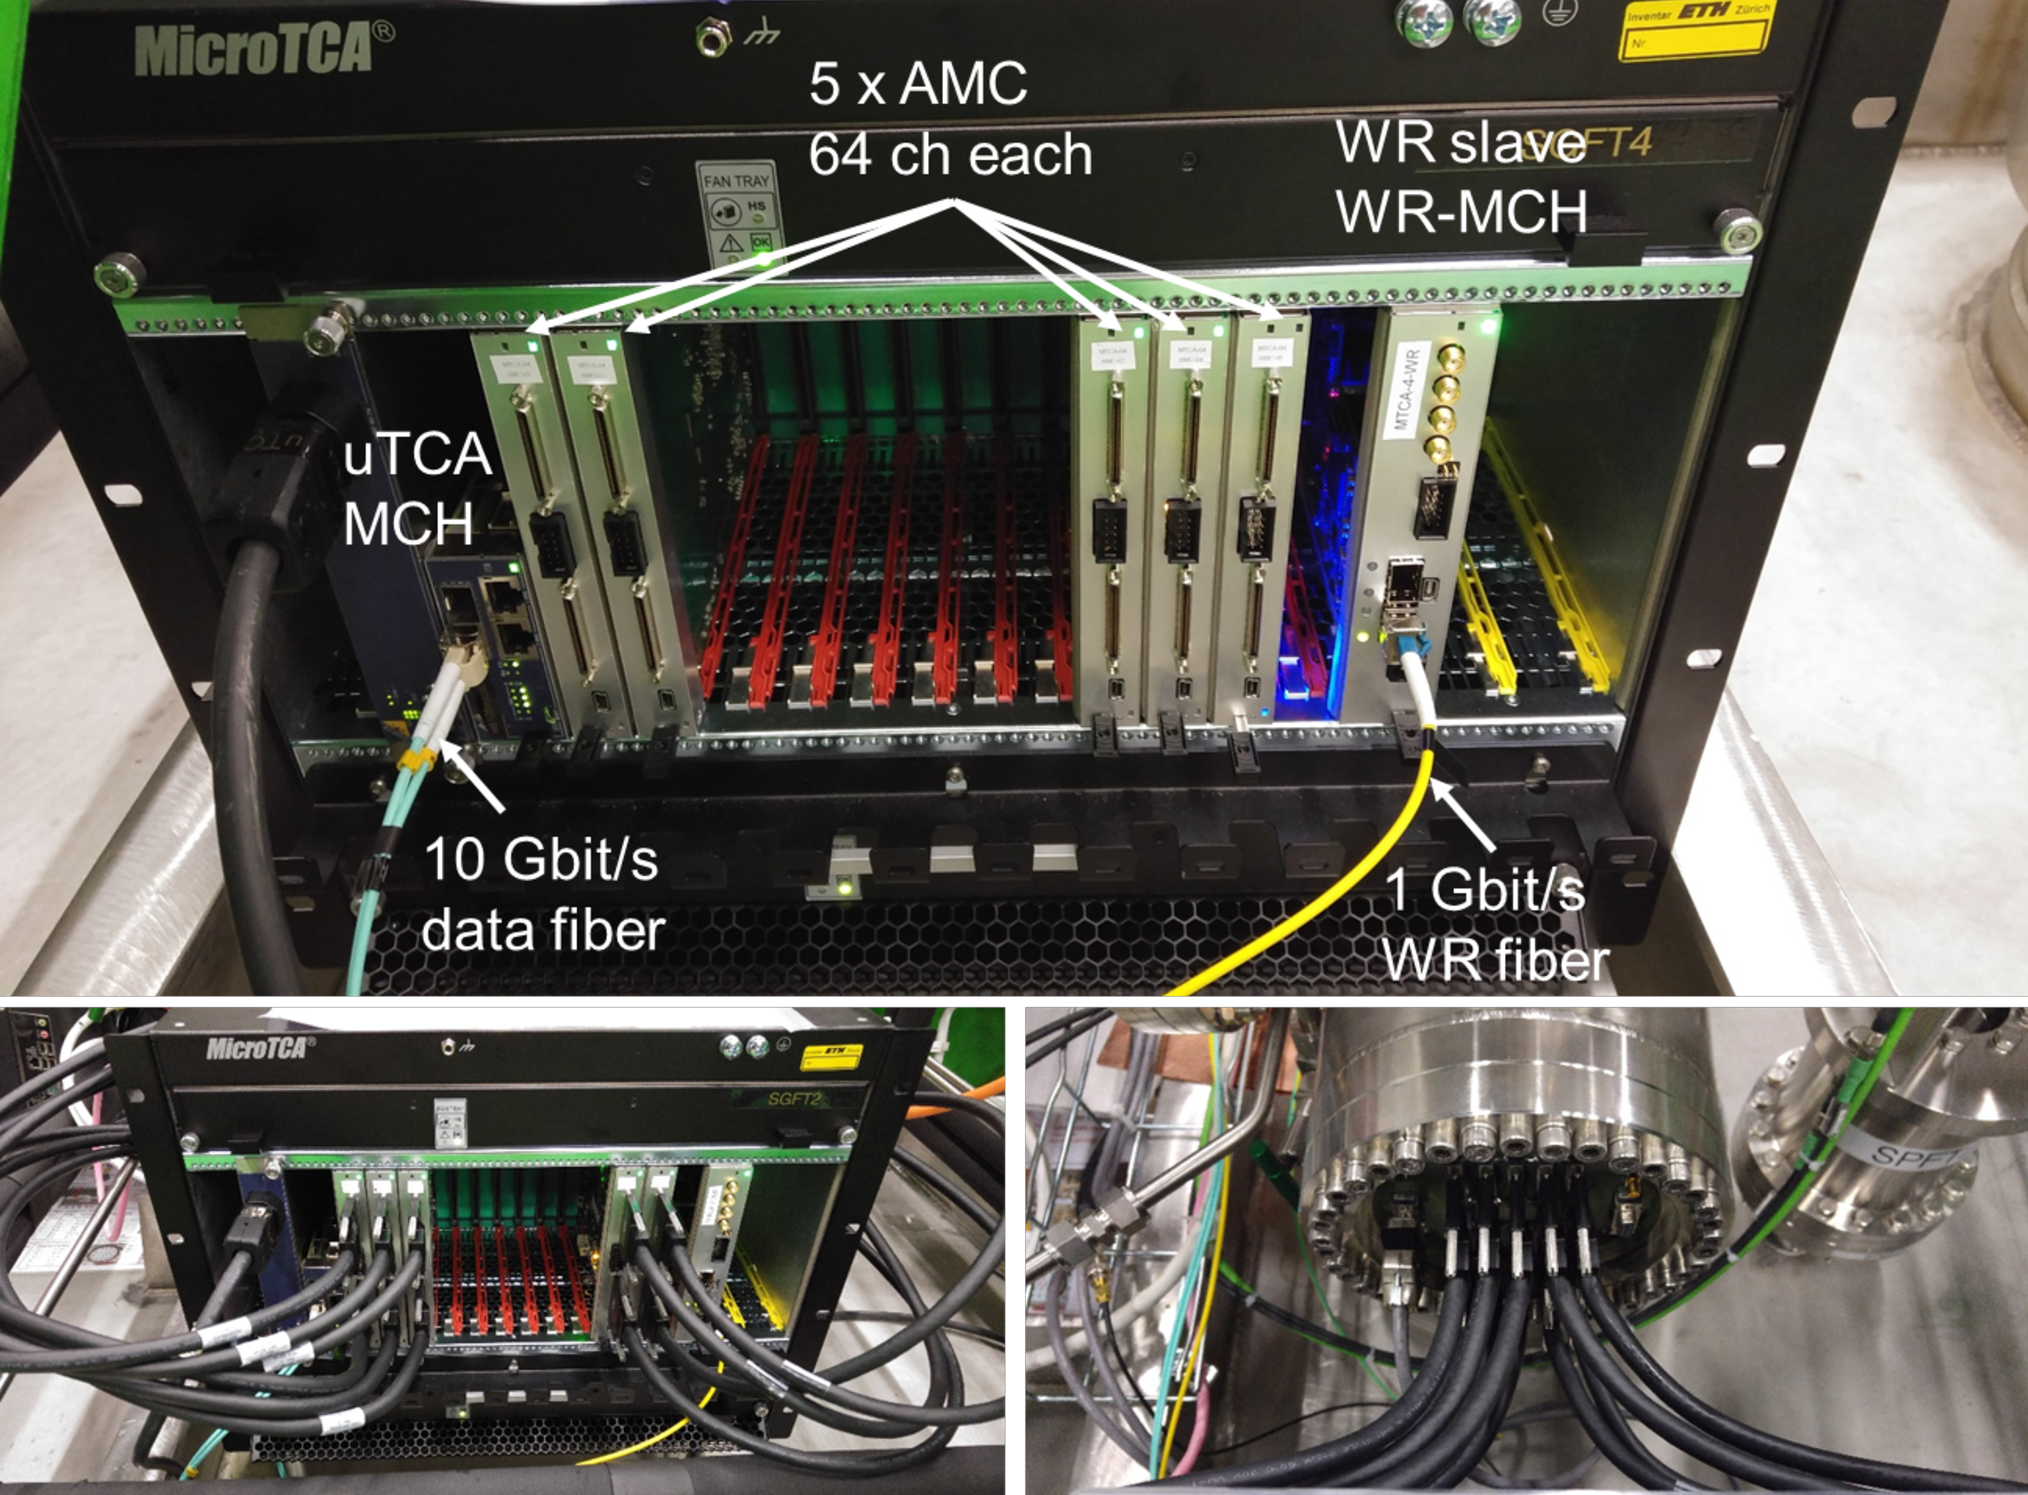
\includegraphics[width=0.6\textwidth]{dpele-311-utca-image}
\end{dunefigure}

In the current design, as used for ProtoDUNE-DP, the MCH operates with a \SI{10}{Gbit/s} uplink. Given that a uTCA crate hosts \num{10} AMCs for charge readout, the required bandwidth to stream the data to DAQ is about \SI{1.8}{Gbit/s}. This assumes that the data exiting AMCs are losslessly compressed with the compression factor of \num{10}. The bandwidth required per crate link for streaming the light readout data is \SI{4.7}{Gbit/s}. The \SI{10}{Gbit/s} MCH is therefore sufficient to support these data rates. However, the technology is moving towards supporting the \SI{40}{Gbit/s} rates. In addition, the channel density per AMC could also be increased for the reason of cost optimizations. For these reasons a move to a \SI{40}{Gbit/s} MCH could be foreseen in the design. This would also imply that the optical links connecting the DAQ system to uTCA MCH should be operable at \SI{40}{Gbit/s}. A summary of the required and supported bandwidths per uTCA crate for continous data streaming is provided in Table~\ref{tab:dp-utcabandwidth}

\begin{dunetable}
[Bandwidth requirements per uTCA crate]
{lr}{tab:dp-utcabandwidth}
{Bandwidth requirements per uTCA crate for continuous data streaming. A compression factor of 10 for the charger readout data is assumed }   
Parameter & Value  \\ \toprowrule
  Charge readout data rate  &  \SI{1.8}{Gbit/s}            \\ \colhline
  Light readout data rate  &  \SI{4.7}{Gbit/s}            \\ \colhline
  Current MCH bandwidth & \SI{10}{Gbit/s} \\ \colhline
  Upgraded MCH bandwidth & \SI{40}{Gbit/s} \\ \colhline
\end{dunetable}

Figure~\ref{fig:dpele-311-utca-image} shows pictures of one of the instrumented uTCA crates used for the charge readout of LArProto at CERN. In this detector each SFT chimney reads \num{320} channels thus requiring only five AMCs per the uTCA crate. The two optical fiber links, one (\SI{10}{Gbit/s}) for data and the other (\SI{1}{Gbit/s}) for clock/trigger timing distribution, are visible in the images.       

%%%%%%%%%%%%%%%%%%%%%%%%%%%%%%%%%%%
\subsection{Timing Distribution}
\label{sec:fddp-tpc-elec-wr}
% WR description and card development
The time synchronization system utilizes a White Rabbit (WR) network, which combines the synchronous 1 Gbit/s Ethernet (SyncE) technology with the exchange of PTPV2 packets, to synchronize clocks of distant nodes to a common time. A high stability GPS disciplined oscillator (GPSDO) with the accuracy similar to that of an atomic clock provides a clock reference signal to be distributed over the physical layer interface of the WR Ethernet network. The network topology is built using specially designed switches that have the standard IEE802.1x Ethernet Bridge functionality with an addition of WR-specific extensions to preserve the clock accuracy. Time and frequency information are distributed to the nodes on the WR network via optical fibers. The WR protocol automatically performs dynamic self-calibrations to account for any propagation delays and keeps all connected nodes continuously synchronized to sub-ns precision. 

The sub-ns accuracy on the clock synchronization is not strictly needed for aligning samples in the different AMC digitization units, since the data have the timing granularity of 400 ns. However, WR timing system offers readily available industrial components and necessary protocols needed for synchronization with automatic calibration of delay propagation and it, therefore, has been adopted. The necessary R\&D for integrating this system with the readout of the ProtoDUNE-DP detector has been completed. 

In the implementation specific to ProtoDUNE-DP, a GPS disciplined clock unit (Meinberg LANTIME M600) feeds 10 MHz and 1 PPS reference signals to a commercial White Rabbit switch (Seven Solutions WRS V3.4). The switch acts as Grand Master of the WR network. It is connected via 1Gbit/s optical links to the dedicated WR timestamping node (WR-TSN) and the WR end-node slave cards present within each uTCA crate (WR-MCH) keeping these synchronized to its reference time. The Grand Master also communicates through a standard Ethernet port with the LANTIME unit for its date and time synchronization via NTP. The WR-TSN module recieves analog TTL-level trigger signals, generates their timestamps, and then transmit these over WR network to the connected WR-MCH units. This timestamp information is then used by AMCs to find the data frame corresponding to the trigger. 

\begin{dunefigure}[Picture of White Rabbit slave WR-MCH card]{fig:dpele-wrmch-image}
{Picture of the WR slave node card (WR-MCH) present in each uTCA crate for time synchronization.The WR-LEN mezzanine card is visible in the bottom right corner}
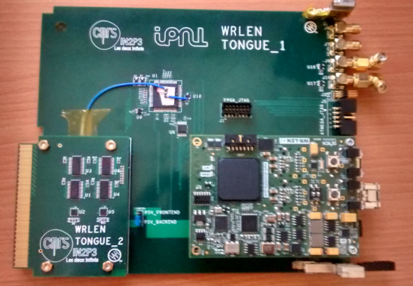
\includegraphics[width=0.45\textwidth]{dpele-wrmch-image}
\end{dunefigure}

The WR-MCH card (Figure~\ref{fig:dpele-wrmch-image}) enables clock/timing/trigger distribution to AMCs. It communicates with them via dedicated lines in the backplane of the uTCA crate using a customized data-frame protocol. The module contains a commercial WR slave node card, the White Rabbit Lite Embedded Node (Seven Solutions OEM WR-LEN), as mezzanine card. WR-LEN runs on a customized firmware which also enables it to decode the trigger timestamp data packet received over the WR network.

\begin{dunefigure}[Architecture of White Rabbit network]{fig:dpele-wrnet-layout}
{Architecture of WR network for time synchronization of digital readout electronics}
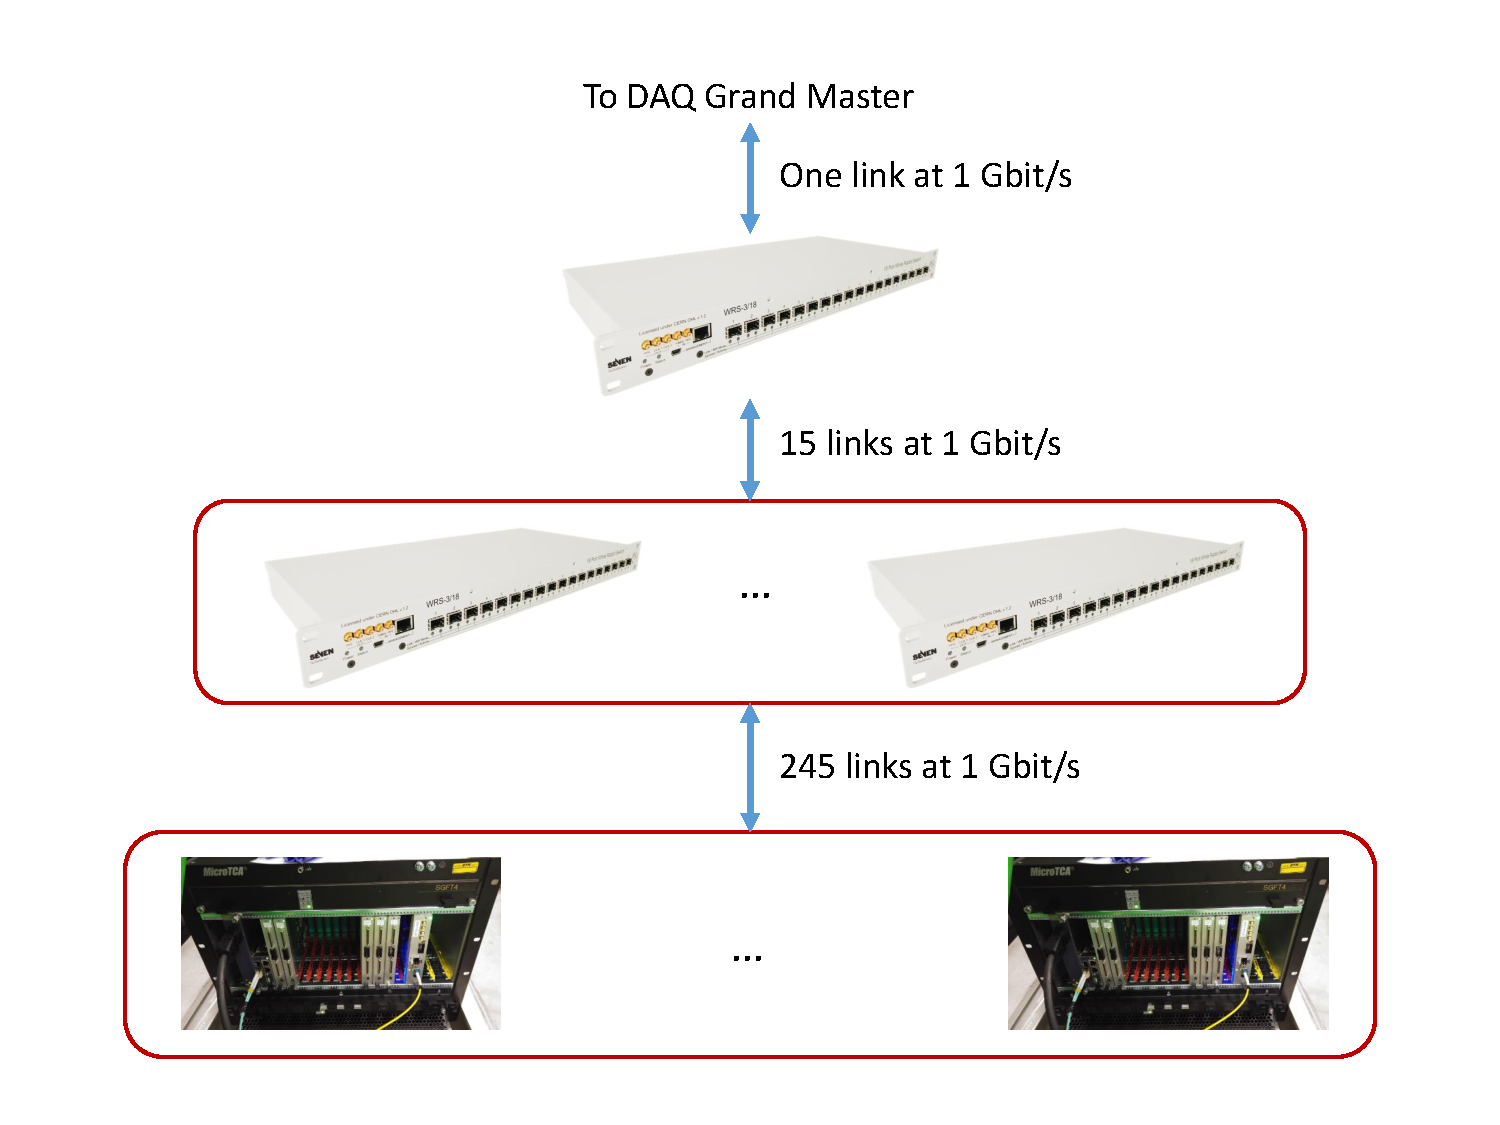
\includegraphics[width=0.7\textwidth]{dpele-wrnet-layout}
\end{dunefigure}

The architecture of the WR network layout for one DP detector module is illustrated Figure~\ref{fig:dpele-wrnet-layout}. It is built in a hierarchical structure from \num{16} WR switches with \num{18} ports each,  chained with \SI{1}{Gbit/s} optical fibers. The switch at the top of the hierarchy interconnects the synchronization Grand Master from the DAQ system with the \num{15} switches in the middle layer. Those are in turn connected to the WR-MCH slave nodes in each uTCA crate (245 in total for charge and light readout). 


%%%%%%%%%%%%%%%%%%%%%%%%%%%%%%%%%%%
\subsection{Electronics for Light Readout}
\label{sec:fddp-tpc-elec-design-lro}

%
The Light Read Out card is a 16-channel AMC; containing one \num{16} channel \num{14} bit \SI{65}{\MHz} ADC (AD9249) and one CatiROC ASIC \cite{catiroc}. A block diagram of the prototype board used for protoDUNE Dual-Phase is shown in Figure \ref{dpele-lro-scheme}. In this prototype, a mezzanine board was developed containing the ASIC and ADC, which sits on a commercial (COTS) mother board (Bittware S4 AMC) containing a high specification FPGA (ALTERA Stratix IV). Figure \ref{dpele-lro-proto} shows the mezzanine and motherboard of the prototype.   For DUNE, one mother board will be produced, merging the mezzannine layout with the mother board developed for the Charge Read out (AMC) and using the ALTERA Cyclone V FPGA. 

Each channel follows two separate paths; the first, through an anti-aliasing low pass filter to be digitized by a \num{14} bit \SI{65}{\MHz} ADC (AD9249), and the second routed directly to the CatiROC ASIC, for precise charge and timing measurements. Both paths will be streamed continuously and independently.

A proposed upgrade is a \num{32} channel card, diminishing the number of cards required and increasing the channel density to 352 channels per uTCA crate.

\begin{dunefigure}[Block diagram of LRO]{fig:dpele-lro-scheme}
{Block diagram of LRO prototype.}
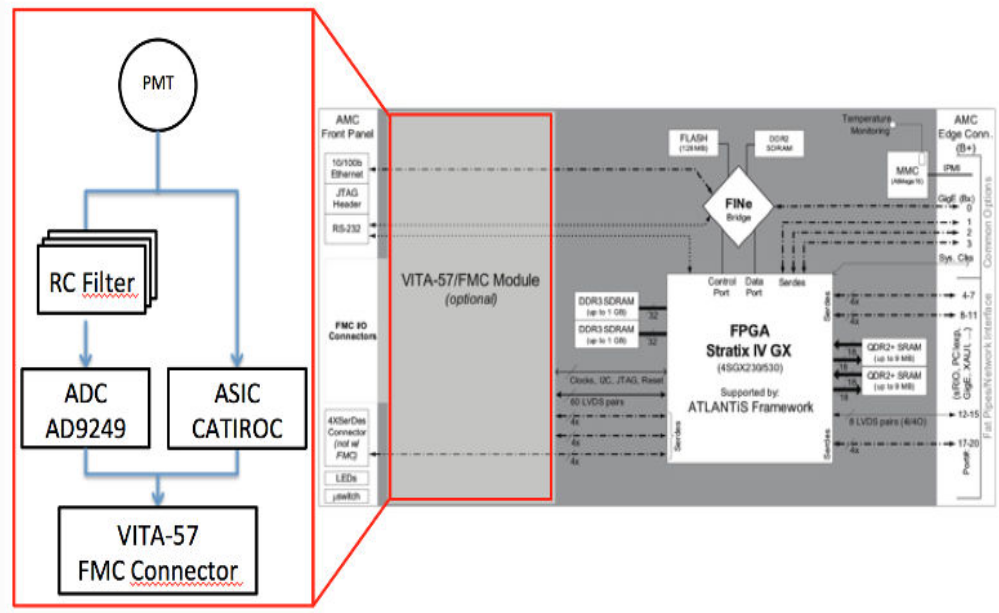
\includegraphics[width=0.7\textwidth]{dpele-lro-scheme}
\end{dunefigure}

\begin{dunefigure}[Prototype LRO card]{fig:dpele-lro-proto}
{The LRO prototype.}
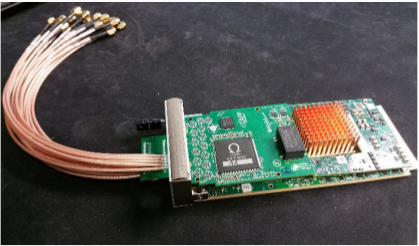
\includegraphics[width=0.7\textwidth]{dpele-lro-proto}
\end{dunefigure}

\subsubsection{Waveform} %ADC
%details on CatiROC
The main characteristics of the ADC are shown in Table \ref{tab:dpele-adc}.

For normal operation, in continuous sampling mode, the time samples will be down-sampled by the FPGA to a coarse \SI{400}{ns} sampling to match that of the Charge Read Out and limit the quantity of data streamed. Before this downsampling, there is the possibility of online pulse processing within the FPGA, to make continuous measurements such as rise and fall times. Even at the coarse sampling of \SI{400}{ns} studies of the liquid argon scintillation time-profile are possible (with the long fall timeconstant of $\sim$\SI{1500}{ns}) and also matching of the electroluminescence signal (also known as proportional scintillation light) to that of the charge signal.  Low light-level signals, such as the single or few photoelectron signals, will show no time structure, but will consist of 1 sample several LSB above the baseline. %err.. is that true??

%RMS and PMT gain?

\begin{dunetable}
[Main characteristics of ADC AD9249.]
{lr} {tab:dpele-adc}
{Main characteristics of the ADC AD9249 used for the Light Read Out}
Item &   \\ \toprowrule
Time resolution & \SI{15}{ns} \\ \colhline
Amplitude resolution (LSB) & \SI{0.122}{mV} \\ \colhline
Dynamic range & \num{14} bit/ \SI{2}{V} \\ \colhline
Differential Non-Linearity & Typical $\pm$\num{0.6} LSB\\
& with Min. \num{-0.9} and Max. \num{+1.6} LSB  \\ \colhline
Integral Non-Linearity & Typical $\pm$\num{0.9}  LSB\\
& with Min. \num{-3} and Max. \num{3} LSB  \\ \colhline
%MEMORY??
\end{dunetable}
%noise llevel??

\subsubsection{Analog Measurements of Charge and Time}%ASIC?

The CATIROC is a \num{16} channel ASIC dedicated to measurement of charge, and precision timing of negative-going PMT signals \cite{Blin:2017}. It auto-triggers on the single photoelectron, and can sustain a high dark rate (up to \SI{20} {kHz/channel}). Charge measurements can be made over the range of \SI{160}{fC} to \SI{70}{pC} (corresponding to approximately to a range of \num{1} - \num{400} photoelectrons with a PMT gain of \num{1E6}). Timing measurements per channel can be made to an accuracy of \SI{200}{ps}.

Figure  \ref{dpele-lro-catiroc} shows the schematic of the ASIC. The slow channel, from which precision charge and timing measurements are made, is formed by two variable gain (8-bit) amplifiers followed by two variable slow shapers; one High Gain for small signals, and one Low Gain for larger signals, and two Track-and-Hold stages. The slow shaper has a tunable shaping time (up to \SI{100}{ns}) and a variable gain.  If the High Gain is saturated, corresponding to passing a pre-determined threshold common to all 16 channels, the Lower Gain value is chosen. The chosen charge value is converted by an internal 10-bit Wilkinson ADC operating at \SI{160}{MHz}.  This slow channel operates in a ping-pong mode, with two capacitors to store the slow shaper signals, giving an effective buffer of 2 events. If both capacitors are full, a deadtime of \SI{5}{\micro\second} arises.

The fast channel is used to auto-trigger the ASIC and make the fine-timing measurement. It comprises a high gain preamplifier, fast shaper (shaping time \SI{5}{ns}) and discriminator which a (\num{10} bit) threshold commmon to the \num{16} channels. The output of the discriminator is used for the two Time to Digital Convertors which form the fine-timing. A coarse timestamp is also obtained by a \num{26} bit counter at \SI{40}{MHz}.  Only channels that resulted in triggers are digitized, their information is transferred to the internal memory ready for read-out by the external FPGA.

%Measurements performed in \cite{Blin2017} ..% SNR of 13 trigger efficiency etc...
%total number of bits per channel, 50-bits from CatiROC?
%COPY CAYETANO TABLE
%SELMA'S SPE FROM JUNO?? or my spe??
\begin{dunefigure}[CatiROC ASIC]{fig:dpele-lro-catiroc}
{Functional diagram of CatiROC ASIC.}
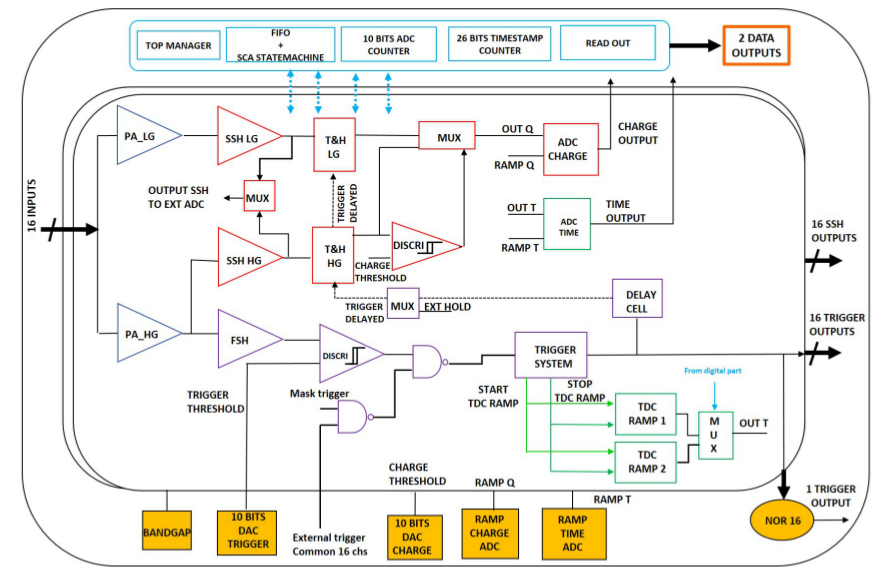
\includegraphics[width=0.7\textwidth]{dpele-lro-catiroc}
\end{dunefigure}

\begin{dunetable}
[Main characteristics of CATIROC.]
{lr} {tab:dpele-catiroc}
{Main characteristics of CATIROC used for the Light Read Out}
Item &   \\ \toprowrule
Number of Channels & \num{16}\\ \colhline
Signal Polarity & negative \\ \colhline
Timing & Time stamp: 26 bit counter at \SI{40}{MHz} \\
       & Fine time: resolution $<$\SI{200}{ps}\\ \colhline
Charge Dynamic Range & \SI{160}{fc} to \SI{100}{pc}\\ \colhline
Trigger & auto-trigger \\
        & Noise= \SI{5}{fC} Minimum threshold = \SI{25}{fC} (5$\sigma$)\\ \colhline
Digital & 10-bit Wilkinson ADC at 160 MHz \\ %TWO READOUT AT 80MHZ??
        & Read-out frame of 50 bits \\ \colhline
Outputs & \num{16} trigger outputs \\
        & NOR16 \\
        & \num{16} slow shaper outputs \\
        & Charge measurement over \num{10} bits \\
        & Time measurements over \num{10} bits \\ \colhline
Main Internal &  Variable preamplifier gain \\
Programmable  &  Variable shaping and gain \\
Features & Common trigger threshold \\
         & Common gain threshold \\ \colhline
\end{dunetable}


%%%%%%%%%%%%%%%%%%%%%%%%%%%%%%%%%%%%%%%%%%%%%%%%%%%%%%%%%%%%%%%%%%%%
\section{Production and Assembly}
\label{sec:fddp-tpc-elec-prod-assy}

%%%%%%%%%%%%%%%%%%%%%%%%%%%%%%%%%%
\subsection{Cryogenic Analog FE Electronics}
\label{sec:fddp-tpc-elec-prod-fe}

%%%%%%%%%%%%%%%%%%%%%%%%%%%%%%%%%%
\subsection{Signal Feedthrough Chimneys}
\label{sec:fddp-tpc-elec-prod-sft}

%%%%%%%%%%%%%%%%%%%%%%%%%%%%%%%%%%
\subsection{Timing System and uTCA}
\label{sec:fddp-tpc-elec-prod-utca}

%%%%%%%%%%%%%%%%%%%%%%%%%%%%%%%%%%
%\subsection{Low-voltage Power Supply System}
%\label{sec:fddp-tpc-elec-prod-lvps}

%%%%%%%%%%%%%%%%%%%%%%%%%%%%%%%%%%%
%\subsection{Digital Electronics}
%\label{sec:fddp-tpc-elec-prod-utca}

\subsection{Charge Readout Electronics}
\label{sec:fddp-tpc-elec-prod-cro}

%%%%%%%%%%%%%%%%%%%%%%%%%%%%%%%%%%%
\subsection{Light Readout Electronics}
\label{sec:fddp-tpc-elec-prod-lro}

%%%%%%%%%%%%%%%%%%%%%%%%%%%%%%%%%
%\subsection{Assembly Procedures}
%\label{sec:fddp-tpc-elec-assy}

%%%%%%%%%%%%%%%%%%%%%%%%%%%%%%%%%%%
\subsection{Quality Assurance}
\label{sec:fddp-tpc-elec-qa}



%%%%%%%%%%%%%%%%%%%%%%%%%%%%%%%%%%%%%%%%%%%%%%%%%%%%%%%%%%%%%%%%%%%%
\section{Interfaces}
\label{sec:fddp-tpc-elec-intfc}

The DP TPC electronics system has interfaces to several other systems. The system must read the charge and light signals from the detector module and thus needs to interface to CRP and the photo-detection systems.  The digitized data must in turn be transmitted to DAQ via the optical links in each uTCA crate. The SFT chimney need to be integrated in the cryostat structure and connected to the cryogenic system. The management of the low-voltage power supplies for the FE analog electronics as well as the monitoring of various sensors in the SFT chimneys have to be part of the slow control. 
\fixme{cite all interface docs?}. 
%\fixme{Include an image of each interface in appropriate section.}

%\fixme{Add in appropriate subsections for the pieces that TPC Electronics interfaces with. These initial ones may not be right.}
\subsection{CRP and Photon Detection System}
\label{sec:fddp-tpc-elec-intfc-crppmt}

The cold flange of the SFT chimneys forms interface between the CRP and the TPC electronics systems. On the side facing the crystostat the flange hosts \num{20} \num{64} pin KEL connectors (XX\todo{part number}) for plugging the flat cables from the CRP. These are 68 channel twisted pair flat cables each carrying signals from \num{32} anode strips and are part of the CRP system. Each analog FE card reads \num{64} anode strips implying receiving signals from two KEL connectors. The order in which the cables are connected into cold flange determines the mapping of the electronic channels to the physical location of the strips on the CRP. This is covered in the greater details in Section~\ref{sec:fddp-tpc-elec-install-sft}. 
\fixme{Perhaps an image of the cold flange showing the connectors?}

\fixme{Interfaces to light readout}


%%%%%%%%%%%%%%%%%%%%%%%%%%%%%%%%%%%
\subsection{DAQ System}
\label{sec:fddp-tpc-elec-intfc-daq}

The hardware interface between DP-Electronics and DAQ has two components. The first interface are the \SI{10}{Gbit/s} optical fibers for data transfer between the uTCA crates and the network interface of the DAQ system. The second one is a \SI{1}{Gbit/s} optical fiber that connects the DAQ White Rabbit Grand Master switch to the DP electronics timing system.   

In the baseline design a given DP detector module would have \num{245} \SI{10}{Gbit/s} optical links for streaming the digitized data to DAQ from the charge readout (\num{240} links) and light light readout (\num{5} links) electronics housed in uTCA crates on top of the cryostat structure.  In the current specifications, the fibers are multimode OM3 fibers\footnote{http://shop.fiber24.net/index.php/en/FO-Patch-Cable-OM3-Multi-mode-50-125-m-Duplex-LC-PC-LC-PC/c-OM3-DUPLEX-1TO1/a-FOPC-F2-O3-DX-LCU-LCU} with LC-LC connectors suitable for the transmission over distances of up to \SI{300}{\metre}.  They are provided by the DAQ consortium. On the side of the uTCA crate, the fibers are connected to an optical transceiver in the MCH\footnote{http://www.nateurope.com/products/NAT-MCH.html} (two SFP+ (XAUI) links).  On the DAQ, they go to the Level 1 (LV1) machines of the trigger farm, or switches, depending on the network topology adopted in the DAQ system design.

The \SI{1}{Gbit/s} link going from the White Rabbit Grand Master to the DP-electronics time distribution network serves to provide the synchronization to the reference clock common for the entire FD. The Grand Master, possibly installed on the surface with the GPSDO (GPS-Disciplined Oscillator) clock unit that receives the GPS signals, distributes the timing information underground over tens of kilometer distance. It automatically compensates for the propagation delays to achieve sub-ns accuracy in the synchronization of the connected slave nodes. The clock information is distributed to the WR-MCH slave module in each uTCA crate via a set of White Rabbit switches. These switches and the interconnecting \SI{1}{Gbit/s} fibers form the timing sub-system of the DP electronics system and are included in the design of the latter.    

The design of the TPC electronics assumes that the data are streamed continuously via the \SI{10}{Gbit/s} links to the DAQ system, where they are buffered until a trigger decision could be made. The triggers are to be issued by processing the buffered data in some suitable sliding time window on the trigger farm machines. The depth of the window may go up to \SI{10}{s} as needed for the definition of the Supernova triggered events. The triggers determine if the data contained in the buffers are to be written on disk. 

The software interface between DAQ and the electronics systems includes the tools dealing with the data transmission and buffering: data formatting in UDP packets, compression/decompression, and exchange of the control packets.

%%%%%%%%%%%%%%%%%%%%%%%%%%%%%%%%%%%
\subsection{Cryostat and Cryogenics}
\label{sec:fddp-tpc-elec-intfc-cryo}

The interface point between the cryostat and the DP electronics system is the cryostat penetrations where the SFT chimneys are to be installed. Each penetration should accommodate the chimney whose external diameter is \SI{245}{\mm}. Each chimney has a CF-273 flange welded to its outer structure (see Figure~\ref{fig:dpele-sft-chimney-crosspipe}). After the chimney is inserted, this flange is in contact with the corresponding flange structure on the cryostat to which it is eventually fastened. In order to avoid any leaks at this interface a CF-273 copper gasket should be used to ensure the vacuum tightness.  

\begin{dunefigure}[Details of SFT chimney interface to the cryostat structure]{fig:dpele-sft-chimney-crosspipe}
{Details of SFT chimney interface to the cryostat structure}
%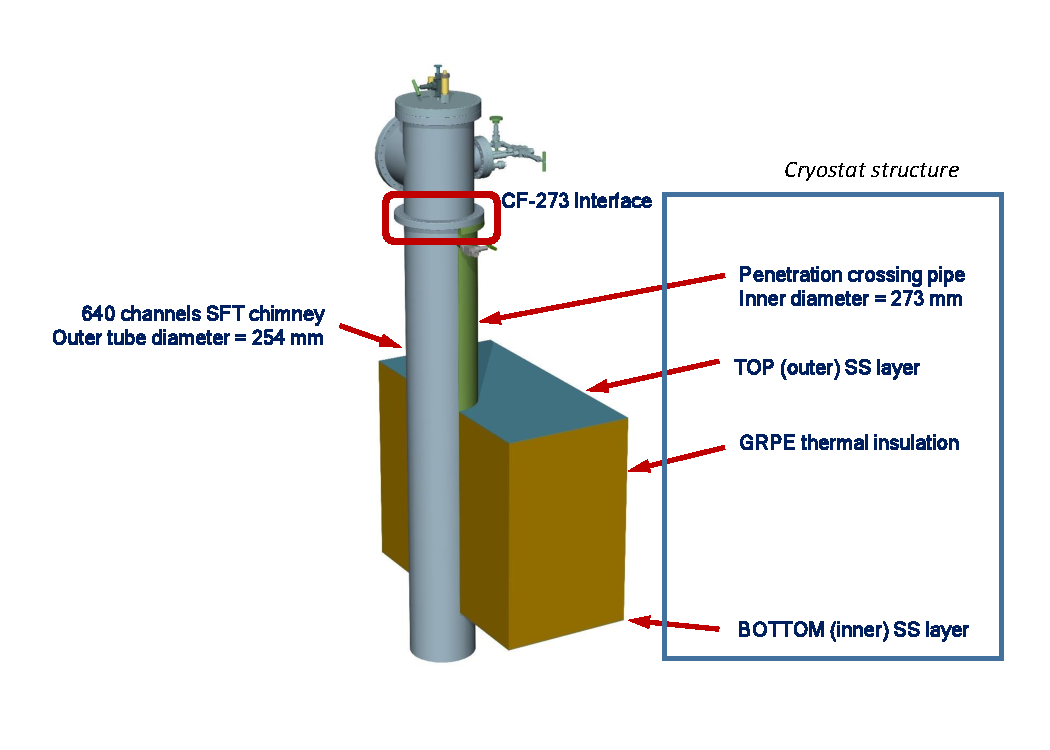
\includegraphics[width=0.7\textwidth]{dpele-sft-chimney-crosspipe}
\end{dunefigure}

Each chimney contains a heat exchanger coil cooled with a liquid argon. There are two \todo{give type and diameter} connections (inlet and outlet) which need to be branched to the respective system for LAr delivery and re-circulation. In addition, there is a connection for nitrogen gas line \todo{give type and diameter}. It is needed for filling the chimney with nitrogen after it is closed following the installation of the FE electronics. The nitrogen line is also required for flushing the chimney in the case of an access to the FE cards after the detector module is cooled for the operation. 

\fixme{say something about clearance need for uTCA crates?}

%%%%%%%%%%%%%%%%%%%%%%%%%%%%%%%%%%%
\subsection{Slow Control System}
\label{sec:fddp-tpc-elec-intfc-sc}

The integration with the slow control of the low voltage power supply system for the FE cards is required to enable the remote management and monitoring (current consumption by ASICs, set voltage, etc.).
In addition, the SFT chimneys contains several sensors that need to be monitored. These include a pressure transducer that measures the pressure inside the chimney and at least two temperature probes (PT1000) that monitor the gas temperature inside near the cold flange at the bottom and close to the warm flange at the top.  

\fixme{other items?}

%%%%%%%%%%%%%%%%%%%%%%%%%%%%%%%%%%%%%%%%%%%%%%%%%%%%%%%%%%%%%%%%%%%%
\section{Installation, Integration and Commissioning}
\label{sec:fddp-tpc-elec-install}

The overall installation sequence...

%%%%%%%%%%%%%%%%%%%%%%%%%%%%%%%%%%%%
\subsection{Transport and Handling}
\label{sec:fddp-tpc-elec-install-transport}

%%%%%%%%%%%%%%%%%%%%%%%%%%%%%%%%%%%
\subsection{Signal Feedthrough Chimneys}
\label{sec:fddp-tpc-elec-install-sft}

%%%%%%%%%%%%%%%%%%%%%%%%%%%%%%%%%%%%
\subsection{Digital uTCA crates}
\label{sec:fddp-tpc-elec-install-utca}

%%%%%%%%%%%%%%%%%%%%%%%%%%%%%%%%%%%%
%\subsection{Infrastructure}
%\label{sec:fddp-tpc-elec-install-cable}

%%%%%%%%%%%%%%%%%%%%%%%%%%%%%%%%%%%
%\subsection{Integration}
%\label{sec:fddp-tpc-elec-install-integ}

%%%%%%%%%%%%%%%%%%%%%%%%%%%%%%%%%%%
\subsection{Integration within DAQ}
\label{sec:fddp-tpc-elec-install-daq}

%%%%%%%%%%%%%%%%%%%%%%%%%%%%%%%%%%%
\subsection{Integration with Photon Detection System}
\label{sec:fddp-tpc-elec-install-pmt}

%%%%%%%%%%%%%%%%%%%%%%%%%%%%%%%%%%%
\subsection{Calibration}
\label{sec:fddp-tpc-elec-install-calib}

%%%%%%%%%%%%%%%%%%%%%%%%%%%%%%%%%%%%%%%%%%%%%%%%%%%%%%%%%%%%%%%%%%%%
\section{Quality Control}
\label{sec:fddp-tpc-elec-qc}

%%%%%%%%%%%%%%%%%%%%%%%%%%%%%%%%%%%%
\subsection{Protection and Assembly (Local)}
\label{sec:fddp-tpc-elec-qc-local}


%%%%%%%%%%%%%%%%%%%%%%%%%%%%%%%%%%%
\subsection{Post-factory Installation (Remote)}
\label{sec:fddp-tpc-elec-qc-remote}


%%%%%%%%%%%%%%%%%%%%%%%%%%%%%%%%%%%%%%%%%%%%%%%%%%%%%%%%%%%%%%%%%%%%
\section{Safety}
\label{sec:fddp-tpc-elec-safety}

%%%%%%%%%%%%%%%%%%%%%%%%%%%%%%%%%%%
% add subsections and labels if needed \subsection{}
%\label{sec:fddp-tpc-elec-safety-}


%%%%%%%%%%%%%%%%%%%%%%%%%%%%%%%%%%
%\subsection{}
%\label{sec:fddp-tpc-elec-safety}


%%%%%%%%%%%%%%%%%%%%%%%%%%%%%%%%%%%%%%%%%%%%%%%%%%%%%%%%%%%%%%%%%%%%
\section{Organization and Management}
\label{sec:fddp-tpc-elec-org}

%%%%%%%%%%%%%%%%%%%%%%%%%%%%%%%%%%%
\subsection{Dual-Phase TPC Electronics Consortium Organization}
\label{sec:fddp-tpc-elec-org-consortium}

The Dual-Phase TPC electronics consortium consists of \num{7} participating institutions from France (\num{3}), Japan (\num{3}), and USA (\num{1}). The consortium leader is Dario Autiero (IPNL, France) and the technical lead is Takuya Hasegawa (KEK, Japan).

%%%%%%%%%%%%%%%%%%%%%%%%%%%%%%%%%%
\subsection{Planning Assumptions}
\label{sec:fddp-tpc-elec-org-assmp}


%%%%%%%%%%%%%%%%%%%%%%%%%%%%%%%%%%%
\subsection{WBS and Responsibilities}
\label{sec:fddp-tpc-elec-org-wbs}

The detailed description of the WBS including the assignments of the responsible institutions could be found in DUNE-doc-5594.

%%%%%%%%%%%%%%%%%%%%%%%%%%%%%%%%%%
\subsection{High-level Cost and Schedule}
\label{sec:fddp-tpc-elec-org-cs}

The detailed cost model has been developed based on the scaling of the costs for the electronics system of ProtoDUNE-DP. It is documented in DUNE-doc-XXXX in addendum.  
